\section{\blue{Failure Theories-NEW PAGE}}

\cyan{BSM: Nice work on this new page. A table at the end summarizing the three main theories and their failure conditions would be a nice addition.}

Failure of a material depends on (1) nature of loading and (2) type of material. There are theories that can predict material failure for complex states. 


\subsection{\red{5.6.1 Types of Material Failure - move here?}}

\subsection{Maximum Shear Stress (Tresca) Criterion}

\noindent If a material is \textbf{ductile}, failure is defined by \textbf{yield stress} ($\sigma_Y$) and occurs at \textbf{max shear stress} ($\tau_{max}$).

\subsubsection{Uniaxial Tension}

\begin{figure*}[!h]
\centering
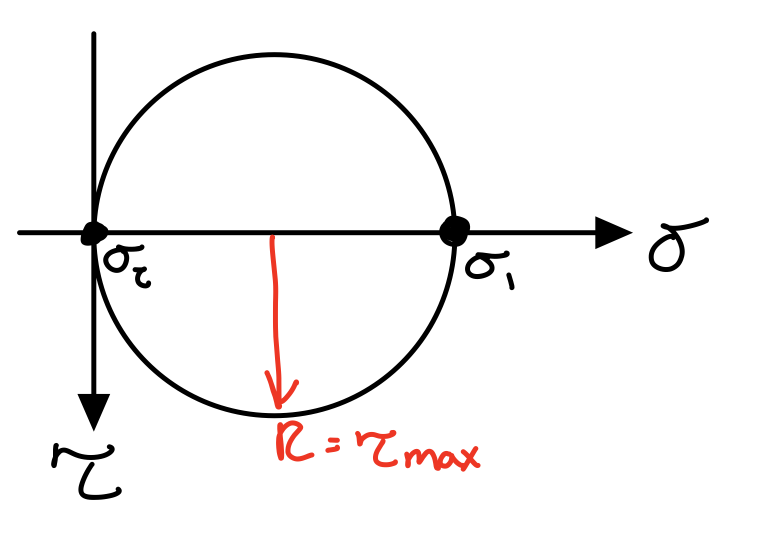
\includegraphics[angle=0, width=2in]{Failure Theories-Figures/Tresca.png}
\vspace{-2mm}
\caption{\small \blue{Taken from TAM251 Lecture Notes - L10S3}}
\vspace{-3mm}
\label{Fig:Tresca}
\end{figure*}

\noindent Consider a material subjected to \textbf{uniaxial tension} $\sigma = \frac{P}{A}$ and $P$ is loaded to the yield point, then the following is true:

\[\sigma_1 = \sigma_Y\]
\[\sigma_2 = 0\]
\[\tau_{max} = \frac{\sigma_Y}{2}\]

\noindent If \textbf{shear stress} is responsible for causing the ductile material to yield, then 

\[\tau_{max} \ge \frac{\sigma_Y}{2}\]

\noindent where $\sigma_Y$ is the \textbf{tensile} yield strength.

\subsubsection{General 2D Loading State}

\[\sigma_z = \sigma_3 = 0\]

\noindent Failure still occurs at 

\[\tau_{max} = \frac{\sigma_Y}{2}\]

\begin{figure*}[!h]
\centering
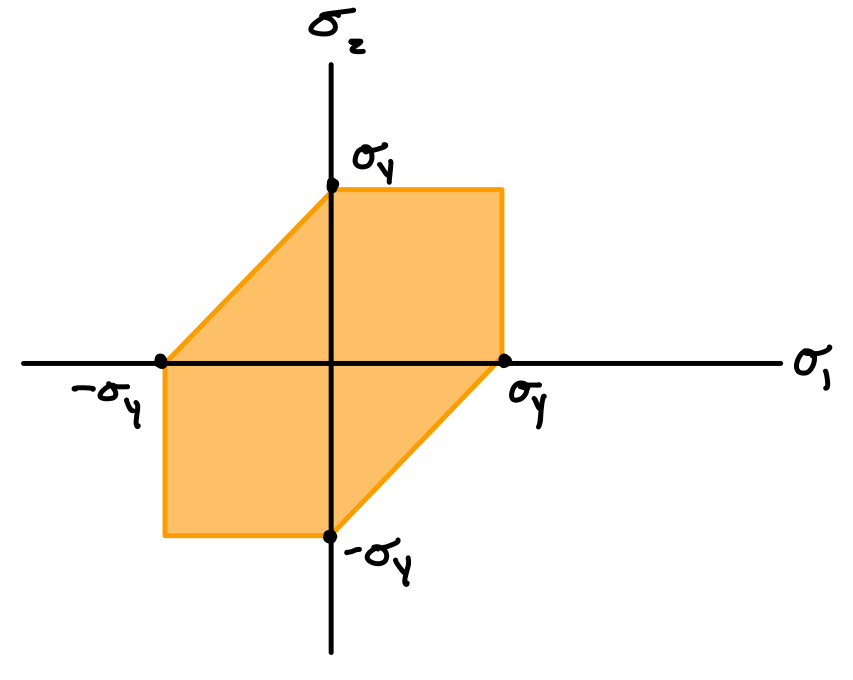
\includegraphics[angle=0, width=3in]{Failure Theories-Figures/TrescaSurface.png}
\vspace{-2mm}
\caption{\small \blue{Taken from TAM251 Lecture Notes - L10S4}}
\vspace{-3mm}
\label{Fig:TrescaSurface}
\end{figure*}

\noindent The equations for $\sigma_1$ and $\sigma_2$ can be plotted to show the failure surface. Loading conditions that occur \textbf{outside} of the surface are when the material fails.

\noindent If $\sigma_1$ and $\sigma_2$ have the \textbf{same} signs

\[|\sigma_1| = \sigma_Y\]
\[|\sigma_2| = \sigma_Y\]

\begin{figure*}[!h]
\centering
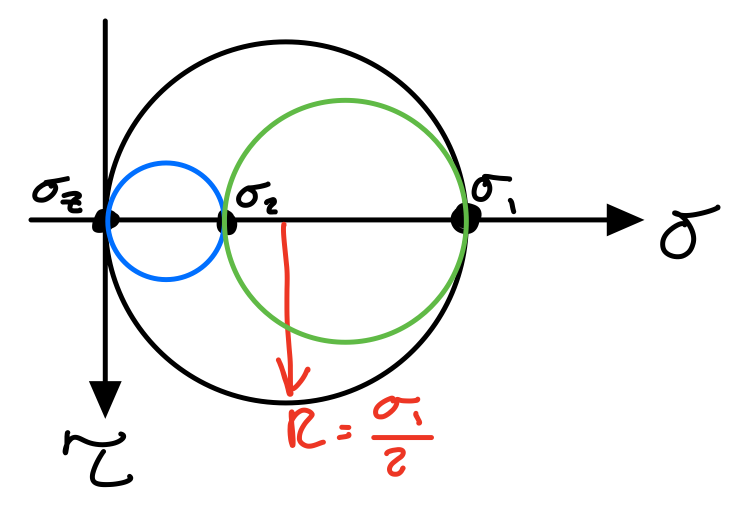
\includegraphics[angle=0, width=2in]{Failure Theories-Figures/TrescaSameSigns.png}
\vspace{-2mm}
\caption{\small \blue{Taken from TAM251 Lecture Notes - L10S5}}
\vspace{-3mm}
\label{Fig:TrescaSame}
\end{figure*}

\noindent If $\sigma_1$ and $\sigma_2$ have \textbf{opposite} signs

\begin{figure*}[!h]
\centering
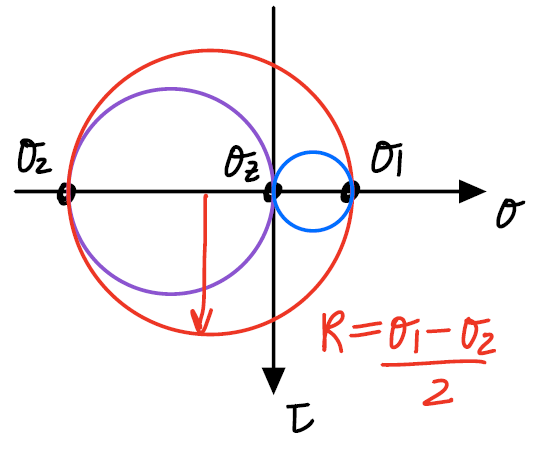
\includegraphics[angle=0, width=2in]{Failure Theories-Figures/TrescaOppositeSigns.png}
\vspace{-2mm}
\caption{\small \blue{Taken from TAM251 Lecture Notes - L10S5}}
\vspace{-3mm}
\label{Fig:TrescaOpp}
\end{figure*}

\[|\sigma_1 - \sigma_2| = \sigma_Y\]

\subsection{Maximum Distortion Energy (Von Misses) Criterion}

\textbf{Ductile} materials likely do not fail due to stresses that only result in a \textbf{volume change}. It is hypothesized that failure is driven by \textbf{distortion strain energy}.

\begin{figure*}[!h]
\centering
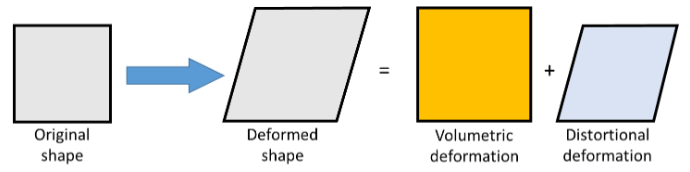
\includegraphics[angle=0, width=4in]{Failure Theories-Figures/VonMises.png}
\vspace{-2mm}
\caption{\small \blue{Taken from TAM251 Lecture Notes - L10S6}}
\vspace{-3mm}
\label{Fig:VonMises}
\end{figure*}

\noindent All elastic deformations can be broken down into \textbf{volumetric} and \textbf{distortional} deformations. 

\vspace{5pt}

\noindent The total strain energy $W$ in a material is broken into these same parts, resulting in

\[W = W_v + W_d\]

\noindent For plane stress
\[W_d = \frac{1+\nu}{3E}(\sigma_1^2 - \sigma_1 \sigma_2 + \sigma_2^2)\]

\noindent At the moment of yield
\[W_{d,yield} = \frac{1+\nu}{3E}\sigma_Y^2\]

\noindent Equating these conditions gives

\[\sigma_1^2 - \sigma_1 \sigma_2 + \sigma_2^2 = \sigma_Y^2\]

\noindent At yield

\[\sigma_{VM}^2 = \sigma_Y^2\]

\noindent Failure occurs at
\[\sigma_{VM} = \sqrt{\sigma_1^2 - \sigma_1 \sigma_2 + \sigma_2^2} \ge \sigma_Y\]


\begin{figure*}[!h]
\centering
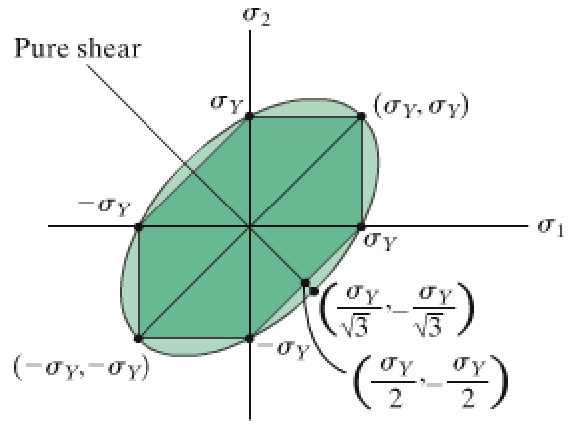
\includegraphics[angle=0, width=3in]{Failure Theories-Figures/VonMisesSurface.png}
\vspace{-2mm}
\caption{\small \blue{Taken from TAM251 Lecture Notes - L10S8}}
\vspace{-3mm}
\label{Fig:VonMisesSurface}
\end{figure*}

\noindent The equating equation be plotted to show the failure surface. The elliptical surface is the Von Mises surface overlaid with the Teresca surface. Loading conditions that occur \textbf{outside} of the surface are when the material fails.

\subsection{Maximum Normal Stress Criterion}

For \textbf{brittle} materials, failure is caused by the \textbf{maximum tensile stress} and NOT compressive stress.

\[|\sigma_1| = \sigma_{ult}\]
\[|\sigma_2| = \sigma_{ult}\]
 
\begin{figure*}[!h]
\centering
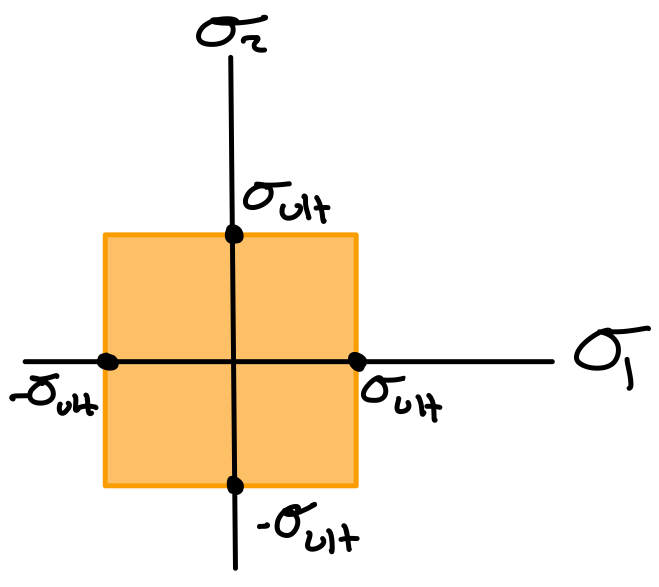
\includegraphics[angle=0, width=3in]{Failure Theories-Figures/Brittle.png}
\vspace{-2mm}
\caption{\small \blue{Taken from TAM251 Lecture Notes - L10S8}}
\vspace{-3mm}
\label{Fig:BrittleFailure}
\end{figure*}

\noindent The $\sigma_1$ and $\sigma_2$ equations can be plotted to show the failure surface. Loading conditions that occur \textbf{outside} of the surface are when the material fails.

\vspace{5pt}

\noindent Brittle fracture can be difficult to predict, so use this theory with caution